\documentclass[aspectratio=169, 10pt]{beamer}

\usepackage{bm} % bold math
\usepackage{fontspec}
\usepackage{minted}
\usepackage{pgf-pie}
\usepackage{tikz}
\usepackage{graphicx}
\newcommand\sbullet[1][.5]{\mathbin{\vcenter{\hbox{\scalebox{#1}{$\bullet$}}}}}

% Custom commands and environments
\makeatletter
\newcommand\version[1]{\renewcommand\@version{#1}}
\newcommand\@version{}
\def\insertversion{\@version}

\newcommand\course[1]{\renewcommand\@course{#1}}
\newcommand\@course{}
\def\insertcourse{\@course}

\newcommand\coursetitle[1]{\renewcommand\@coursetitle{#1}}
\newcommand\@coursetitle{}
\def\insertcoursetitle{\@coursetitle}

\newcommand\lecturenumber[1]{\renewcommand\@lecturenumber{#1}}
\newcommand\@lecturenumber{}
\def\insertlecturenumber{\@lecturenumber}
\makeatother

\newcommand{\slidetitle}[1]{{\xbseries \large \structure{#1}} \bigskip}
\newcommand{\term}[1]{{\color{blue} #1}}
\newcommand{\leftspace}{\hspace{1em}}
\newcommand{\inlinearrow}{
  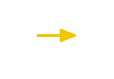
\begin{tikzpicture}[baseline]
    \node [anchor=base] (x) {};
    \draw [rawarrow] (x.mid west) -- ($(x.mid west) + (2em,0)$);
  \end{tikzpicture}
}

\newenvironment{slide}
{\begin{frame}[fragile,environment=slide]\vskip0pt plus 1filll}
{\vskip0pt plus 1filll\end{frame}}

% LaTeX

\setlength{\leftmargini}{1em}

% Common Information

\author{Talia Xu}
\course{COMPSCI 340}
\coursetitle{Operating Systems}
\date{2024 Semester 2}

% fontspec

\defaultfontfeatures{Ligatures=TeX}
% \setmainfont{Domine}
\setsansfont{Inter}[
  FontFace={ul}{n}{Font=*-Thin},
  FontFace={el}{n}{Font=*-ExtraLight},
  FontFace={l}{n}{Font=*-Light},
  FontFace={sb}{n}{Font=*-SemiBold},
  FontFace={eb}{n}{Font=*-ExtraBold},
  FontFace={xb}{n}{Font=*-Black},
]
\setmonofont[Contextuals=AlternateOff, Ligatures=TeXOff]{Iosevka}[
  FontFace={xb}{n}{Font=*-Heavy},
]

%% Font Weights

\DeclareRobustCommand{\ulseries}{\fontseries{ul}\selectfont}
\DeclareTextFontCommand{\textul}{\ulseries}
\DeclareRobustCommand{\elseries}{\fontseries{el}\selectfont}
\DeclareTextFontCommand{\textel}{\elseries}
\DeclareRobustCommand{\lseries}{\fontseries{l}\selectfont}
\DeclareTextFontCommand{\textl}{\lseries}
\DeclareRobustCommand{\sbseries}{\fontseries{sb}\selectfont}
\DeclareTextFontCommand{\textsb}{\sbseries}
\DeclareRobustCommand{\ebseries}{\fontseries{eb}\selectfont}
\DeclareTextFontCommand{\texteb}{\ebseries}
\DeclareRobustCommand{\xbseries}{\fontseries{xb}\selectfont}
\DeclareTextFontCommand{\textxb}{\xbseries}

% tikz

\usetikzlibrary{
  arrows,
  arrows.meta,
  automata,
  backgrounds,
  calc,
  decorations.pathreplacing,
  matrix,
  positioning,
  overlay-beamer-styles,
  shapes,
  shapes.multipart,
  tikzmark,
}

\tikzstyle{rawarrow} = [
  -{Latex[round]},
  line width=1pt,
  yellow,
  shorten >=3pt,
  shorten <=3pt,
  font=\small,
  text=black,
]

\tikzstyle{arrow} = [
  -{Latex[round]},
  line width=1pt,
  yellow,
  shorten >=3pt,
  shorten <=3pt,
  transform canvas={yshift=3pt},
  font=\small,
  text=black,
]

\newcommand{\tikzmarkcoord}[1]{([yshift=3pt]pic cs:#1)}

% minted

\setminted{style=eyolfson, fontsize=\small, escapeinside=||}
\setmintedinline{fontsize=\normalsize}

% hyperref

\hypersetup{colorlinks, urlcolor=blue}

% beamer
\setbeamersize{text margin left=16mm, text margin right=16mm}
\setbeamertemplate{itemize items}[circle]
\setbeamercolor{item}{fg=black}
\setbeamercolor{structure}{fg=darkblue}
\setbeamerfont{frametitle}{series=\bfseries, parent=structure}
\setbeamertemplate{navigation symbols}{}
\setbeamertemplate{headline}{}
\setbeamertemplate{footline}{
  \begin{tikzpicture}[
    remember picture,
    overlay,
    shift={(current page.south west)},
  ]
    \path [fill=gray] (144mm, 0) -- (160mm, 16mm) -- (160mm, 0);
    \node [inner sep=3.5mm, outer sep=0, text=black, anchor=base east,
           align=right, yshift=3.5mm]
          at (current page.south east) {\ttfamily \small \insertframenumber{}};
  \end{tikzpicture}
}
\setbeamertemplate{title page}{
  \begin{tikzpicture}[
    remember picture,
    overlay,
    shift={(current page.south west)},
    background rectangle/.style={fill=darkblue},
    show background rectangle,
  ]
    \node [anchor=center, align=center, text=white, text width=40mm, scale=3.2]
          at (\paperwidth / 2, \paperheight * 2 / 3)
          {\xbseries \inserttitle{}};
    \node [anchor=base west, align=left, inner sep=0, text=white, yshift=2.5mm]
          at (16mm, \paperheight / 3)
          {\insertdate{} \insertcourse{}: \insertcoursetitle{}};
    \node [anchor=base west, align=left, inner sep=0, text=white, yshift=-2.5mm]
          at (16mm, \paperheight / 3)
          {\insertauthor};
    \node [anchor=base east, align=right, inner sep=0, text=white, yshift=2.5mm]
          at (144mm, \paperheight / 3)
          {Lecture \insertlecturenumber{}};
    \node [anchor=base east, align=right, inner sep=0, text=white,
           yshift=-2.5mm]
          at (144mm, \paperheight / 3)
          {\ttfamily \insertversion{}};
    \node [align=center, anchor=south, inner sep=0, text=white, yshift=3.5mm]
          (license) at (\paperwidth / 2, 0)
          {\fontsize{7pt}{7pt}\selectfont This  work is licensed under a
           \href{http://creativecommons.org/licenses/by-sa/4.0/}
                {\color{lightblue} Creative Commons Attribution-ShareAlike 4.0
                 International License}};
  \end{tikzpicture}
}

% xcolor

%% Primary Colour

\definecolor{pantone655}{RGB}{0, 42, 92} % #002a5c
\colorlet{darkblue}{pantone655}

%% Secondary Colours

\definecolor{pantone633}{RGB}{0, 139, 176} % #008bb0
\colorlet{blue}{pantone633}

\definecolor{pantonewarmred}{RGB}{220, 70, 51} % #dc4633
\colorlet{red}{pantonewarmred}

\definecolor{pantone3285}{RGB}{0, 161, 137} % #00a189
\colorlet{cyan}{pantone3285}

\definecolor{pantone7722}{RGB}{13, 83, 77} % #0d534d
\colorlet{darkcyan}{pantone7722}

\definecolor{pantone376}{RGB}{141, 191, 46} % #8dbf2e
\colorlet{green}{pantone376}

\definecolor{pantone2613}{RGB}{109, 36, 122} % #6d247a
\colorlet{violet}{pantone2613}

\definecolor{pantone2985}{RGB}{111, 199, 234} % #6fc7ea
\colorlet{lightblue}{pantone2985}

\definecolor{pantone227}{RGB}{171, 19, 104} % #ab1368
\colorlet{magenta}{pantone227}

\definecolor{pantone7406}{RGB}{241, 197, 0} % #f1c500
\colorlet{yellow}{pantone7406}

%% Neutrals

\definecolor{pantonecoolgray2}{RGB}{208, 209, 201} % #d0d1c9
\colorlet{gray}{pantonecoolgray2}


\lecturenumber{7}
\title{Process Practice}
\version{2.0.0}

\begin{document}
  \begin{frame}[plain, noframenumbering]
    \titlepage
  \end{frame}

  \begin{slide}
    
    \slidetitle{A Teaching Operating System}

    \url{https://github.com/mit-pdos/xv6-riscv}
    \medskip

    Used in MIT graduate OS courses, it is a full OS you can run on the VM

    \leftspace{}You'll run it as a VM using QEmu (yes, a VM in a VM)
    \bigskip
  
    It's a re-implementation of Unix version 6 for RISC-V in C
  \end{slide}

  \begin{slide}

    \slidetitle{Uniprogramming is for Old Batch Processing OSs}

    Uniprogramming: only one process running at a time

    \leftspace{}Two processes are not parallel and not concurrent, no matter
                 what
    \medskip

    Multiprogramming: allow multiple processes

    \leftspace{}Two processes can run in parallel or concurrently
    \bigskip

    Modern operating systems try to run everything in parallel and concurrently
  \end{slide}

  \begin{slide}
    \slidetitle{The Scheduler Decides When To Switch}

    To create a process, the operating system has to at least load it into memory
    \medskip

    When it's waiting, the scheduler (coming later) decides when it's running
    \medskip

    We're going to first focus on the mechanics of switching processes
  \end{slide}

  \begin{slide}
    \slidetitle{The Core Scheduling Loop Changes Running Processes}

    \begin{enumerate}
      \item Pause the currently running process 
      \item Save its state, so you can restore it later
      \item Get the next process to run from the scheduler
      \item Load the next process' state and let that run
    \end{enumerate}
  \end{slide}

  \begin{slide}
    \slidetitle{We Can Let Processes Themselves, or the Operating System Pause}
    
    Cooperative multitasking

    \leftspace{}The processes use a system call to tell the operating system to
    pause it
    \medskip

    True multitasking

    \leftspace{}The operating system retains control and pauses processes
    \bigskip

    For true multitasking the operating system can:
    \begin{itemize}
      \item Give processes set time slices
      \item Wake up periodically using interrupts to do scheduling
    \end{itemize}
  \end{slide}

  \begin{slide}
    
    \slidetitle{Swapping Processes is called Context Switching}

    We've said that at minimum we'd have to save all the current registers

    \leftspace{}We have to save all the values, using the same CPU as we're
    trying to save
    \medskip

    There's hardware support for saving state, however you may not want to save
    everything
    \medskip

    Context switching is pure overhead, we want it to be as fast as possible
    \bigskip

    Usually there's a combination of hardware and software to save as little as
    possible
  \end{slide}

  \begin{slide}
    \slidetitle{A New API --- \texttt{pipe}}

    \mintinline{c}{int pipe(int pipefd[2]);}
    \medskip

    Returns \texttt{0} on success, and \texttt{-1} on failure
    (and sets \texttt{errno})
    \medskip

    \texttt{pipe} forms a one-way communication channel using two file
    descriptors

    \leftspace{}\texttt{pipefd[0]} is the \texttt{read} end of the pipe

    \leftspace{}\texttt{pipefd[1]} is the \texttt{write} end of the pipe
    \medskip

    You can think of it as a kernel managed buffer

    \leftspace{}Any data written to one end can be read on the other end
  \end{slide}

  \begin{slide}
    
    \slidetitle{Aside: Using \& in Your Shell}

    If you use \& at the end of your command, your shell will start that
    process and return

    \leftspace{}e.g. \mintinline{c}{sleep 1 &}
    \medskip

    It outputs the \mintinline{c}{pid} and lets you know when it's finished
    \medskip

    The \mintinline{c}{|} character creates a pipe between two processes
    \medskip

    The sneaky Bash fork bomb is: \mintinline{c}{:(){ :|:& };:}

    \leftspace{}{\color{pantonewarmred} \bfseries Do not run this command}
  \end{slide}

  \begin{slide}
    
    \slidetitle{Let's See the Example}

    See: \texttt{07-process-practice/pipes.c}
    \medskip

    If we remove the call to \texttt{write} in the parent, the child never exits
    \medskip

    What happens to the child?
  \end{slide}


  \begin{slide}
    
    \slidetitle{Final 2022 Question 1}

    For each program shown below, state whether it will produce the
    \textbf{same} output each time it is run, or whether it may produce
    \textbf{different} outputs when run multiple times.
    Explain why the program behaves like this.
    \medskip

    \begin{minted}{c}
int main() {
  int i = 4;
  while (i != 0) {
    int pid = fork();
    if (pid == 0) {
      i--;
    }
    else {
      printf("%d\n", i);
      exit(0);
    }
  }
  return 0;
}
    \end{minted}
  \end{slide}

  \begin{slide}
    
    \slidetitle{Final 2022 Question 2}

    Same as the previous question, except now there's a \texttt{waitpid}
    \medskip

    \begin{minted}{c}
int main() {
  int i = 4;
  while (i != 0) {
    int pid = fork();
    if (pid == 0) {
      i--;
    }
    else {
      waitpid(pid, NULL, 0);
      printf("%d\n", i);
      exit(0);
    }
  }
  return 0;
}
    \end{minted}
  \end{slide}

\end{document}
